% !TeX root = ../main.tex

The experiments is this study were conducted using a widely recognized credit card dataset that includes transactions made by European cardholders in September 2013. This dataset contains 492 fradulent transactions out of a total of 284,807 transactions recorded over two days. Since fraction of fraudulent transactions is extremely low (0.172\%), this dataset presents a highly imbalanced.

The selection of algorithms for fraud detection and classification using the credit card dataset employs a diverse array of methods to tackle the challange posed by its significant imbalance. The selected algorithms comprise machine learning models: LR, DT, RF, XGBoost, SVM, KNN, and GaussianNB.

\section*{Research questions}
\begin{itemize}
    \item Which ML/DL models deliver the strongest fraud-detection performance on imbalanced European credit-card datasets \cite{kaggle_dataset}, and how do they compare when augmented by different balancing and feature-selection strategies?
    \item How does feature selection (e.g., LDA, PCA, GA-based selectors) impact model performance and interpretability?
\end{itemize}

\section*{Data sources}
European credit card dataset \cite{kaggle_dataset} (the standard 30 features V1–V28, Time, Amount; fraud label). Use the original data with preprocessing as a baseline, and also consider a SMOTE/ADASYN-augmented version for comparison.

\section*{Experimental design}
\begin{description}
    \item \textbf{Baseline models:} Logistic Regression (\acrshort{lr}), Decision Tree (\acrshort{dt}), Random Forest (\acrshort{rf}), XGBoost (\acrshort{xgboost}), SVM (\acrshort{svm}), K-Nearest Neighbors (\acrshort{knn}), Gaussian Naive Bayes (\acrshort{gaussiannb}) as a \acrlong{ml} baseline.
    \item \textbf{Feature handling:} Standardize features.
    \item \textbf{Balancing strategies:}
        \begin{itemize}
            \item No resampling (baseline on original data)
            \item Classic oversampling (SMOTE, ADASYN)
            \item Deep generative oversampling (GAN)
            \item Undersampling methods as a complement for comparison (careful handling to avoid loss of information)
        \end{itemize}
    \item \textbf{Model optimization:}
        \begin{itemize}
            \item Hyperparameter tuning for each model (regularization, tree depth, learning rate, number of trees, kernel parameters, etc.)
            \item Cross-validation (e.g., stratified k-fold) to ensure robustness.
        \end{itemize}
    \item \textbf{Evaluation metrics:}
        \begin{itemize}
            \item \textbf{Primary:} AUC/ROC, F1-score, recall (fraud detection emphasis), precision
            \item \textbf{Secondary:} Accuracy, PR-AUC
            \item Computational metrics: training time, inference latency (for real-time considerations)
        \end{itemize}
    \item \textbf{Validation strategy:}
        \begin{itemize}
            \item Stratified k-fold cross-validation for robust estimates
            \item Holdout test set for final evaluation
            \item Statistical significance testing (e.g., paired t-tests or non-parametric tests) to compare top models
        \end{itemize}
    \item \textbf{Reproducibility:} Document seeds, data preprocessing steps, and exact hyperparameters; consider releasing code and configuration files.
    \item \textbf{Data analysis plan:}
        \begin{itemize}
            \item Compare performance across models and balancing strategies using aggregated metrics (mean and 95\% CIs) over cross-validation folds.
            \item Analyze feature importance and model explainability (SHAP values or feature-importance plots for tree ensembles; LIME for select models).
            \item Investigate the impact of feature selection by comparing performance with and without FS, and by analyzing the most informative features across models.
            \item Evaluate robustness to distribution shifts by testing models trained on European data on the second dataset without retraining, then with retraining.
        \end{itemize}
    \item \textbf{Deliverables:}
        \begin{itemize}
            \item A comprehensive experimental report detailing methodology, results, and interpretations.
            \item Clear figures and tables showing model performance across configurations.
            \item An Abbreviations section and a Findings/Recommendations section suitable for the dissertation narrative.
        \end{itemize}
    \item \textbf{Tools and environment :}
        \begin{itemize}
            \item Python-based ML stack (scikit-learn for baseline models; XGBoost or LightGBM for gradient-boosted trees; TensorFlow/Keras or PyTorch for DL baselines; imbalanced-learn for SMOTE/ADASYN).
            \item \textbf{Data visualization:} matplotlib/seaborn for performance plots; SHAP for interpretability.
            \item \textbf{Reproducibility:} Jupyter/Notebook pipelines with requirements.txt; a reproducible workflow (e.g., Makefile or a simple Python script with config files).
            \item Version control (Git) for code management.
        \end{itemize}
\end{description}

% ================================
% Machine Learning Models Section
% ================================
\section*{Machine Learning Models Used in This Study}

    \subsection*{Logistic Regression (LR)}
    Logistic Regression is a supervised binary classifier that models the probability of a transaction being fraudulent. 
    Given an input vector $x = [x_1, x_2, \dots, x_n]$, the model computes a linear combination:
    \[
    z = w_0 + \sum_{i=1}^{n} w_i x_i
    \]
    The probability of fraud is obtained using the sigmoid function:
    \[
    P(\text{fraud} \mid x) = \sigma(z) = \frac{1}{1 + e^{-z}}
    \]
    Model training minimizes the binary cross-entropy loss:
    \[
    L = -\frac{1}{m}\sum_{j=1}^{m} \left[ y_j \log(\hat{y}_j) + (1 - y_j)\log(1 - \hat{y}_j) \right]
    \]

    % ----------------------------------------

    \subsection*{Na\"ive Bayes (NB)}
    Na\"ive Bayes is a probabilistic classifier based on Bayes' theorem with an independence assumption among features. 
    The posterior probability for class $C_k$ is computed as:
    \[
    P(C_k \mid x) = \frac{P(x \mid C_k) P(C_k)}{P(x)}
    \]
    For Gaussian Na\"ive Bayes, each feature follows:
    \[
    P(x_i \mid C_k) = \frac{1}{\sqrt{2\pi\sigma_{ki}^2}} 
    \exp\left( -\frac{(x_i - \mu_{ki})^2}{2\sigma_{ki}^2} \right)
    \]

    % ----------------------------------------

    \subsection*{Decision Tree (DT)}
    Decision Trees recursively split the data into partitions by selecting the feature that maximizes information gain. 
    Node impurity is computed using the Gini index:
    \[
    Gini = 1 - \sum_{i=1}^{C} p_i^2
    \]
    Decision Trees are interpretable but prone to overfitting, especially on imbalanced datasets.

    % ----------------------------------------

    \subsection*{Random Forest (RF)}
    Random Forest is an ensemble model consisting of multiple Decision Trees trained on bootstrap samples.
    The final prediction is obtained by majority voting:
    \[
    \hat{y} = \text{mode}( h_1(x), h_2(x), \dots, h_T(x) )
    \]
    where $h_t(x)$ is the prediction of the $t^{th}$ tree. 
    Random Forest reduces variance and improves robustness.

    % ----------------------------------------

    \subsection*{k-Nearest Neighbors (KNN)}
    KNN classifies a data point based on the majority label among its $k$ nearest neighbors using Euclidean distance:
    \[
    d(x, x_j) = \sqrt{\sum_{i=1}^n (x_i - x_{ji})^2}
    \]
    The predicted label is:
    \[
    \hat{y} = \text{mode}(y_1, y_2, \dots, y_k)
    \]

    % ----------------------------------------

    \subsection*{XGBoost (Extreme Gradient Boosting)}
    XGBoost builds trees sequentially, where each new tree corrects previous residuals. 
    Its regularized objective function is:
    \[
    \mathcal{L} = \sum_{i=1}^{m} l(y_i, \hat{y}_i^{(t)}) + \sum_{k=1}^{t} \Omega(f_k)
    \]
    with:
    \[
    \Omega(f) = \gamma T + \frac{1}{2} \lambda \sum_{j=1}^{T} w_j^2
    \]
    Model predictions are updated iteratively as:
    \[
    \hat{y}_i^{(t)} = \hat{y}_i^{(t-1)} + \eta f_t(x_i)
    \]

    % ----------------------------------------

    \subsection*{LightGBM (LGBM)}
    LightGBM is a gradient boosting framework designed for efficiency using histogram-based learning and leaf-wise tree growth.
    The split gain is computed as:
    \[
    Gain = \frac{1}{2} \left( 
    \frac{G_L^2}{H_L + \lambda} + 
    \frac{G_R^2}{H_R + \lambda} - 
    \frac{(G_L + G_R)^2}{H_L + H_R + \lambda}
    \right)
    \]
    where $G$ and $H$ represent gradient and Hessian statistics.

% ================================
% Balancing Techniques
% ================================

\section*{Balancing Techniques}

    \subsection*{SMOTE (Synthetic Minority Oversampling Technique)}
    SMOTE creates new synthetic minority samples by interpolating between a sample $x$ and one of its nearest neighbors $x_{nn}$:
    \[
    x_{\text{new}} = x + \delta (x_{nn} - x), \quad \delta \sim U(0,1)
    \]

    % ----------------------------------------

    \subsection*{GAN-Based Oversampling}
    A Generative Adversarial Network consists of a generator $G$ and discriminator $D$ trained in an adversarial manner.

    Generator output:
    \[
    G(z; \theta_g) \rightarrow x_{\text{fake}}
    \]

    Discriminator objective:
    \[
    D(x) = P(\text{real} \mid x)
    \]

    GAN training optimizes:
    \[
    \min_G \max_D V(D,G) = 
    \mathbb{E}_{x \sim p_{data}}[ \log D(x) ] 
    + \mathbb{E}_{z \sim p_z}[ \log(1 - D(G(z))) ]
    \]

% ================================
% Algorithm
% ================================

\begin{algorithm}[H]
    \caption{Workflow of the Proposed Methodology}
    \begin{algorithmic}[1]

        \State \textbf{Step 1:} Load the dataset.

        \State \textbf{Step 2: Data Cleaning}
            \Statex \quad Remove inconsistencies, handle missing values, and ensure data integrity.

        \State \textbf{Step 3: Train--Test Split}
            \Statex \quad Split the dataset into training and testing subsets.

        \State \textbf{Step 4: Feature Scaling}
            \Statex \quad Normalize or standardize numerical features.

        \State \textbf{Step 5: Resampling}
            \Statex \quad Address class imbalance using SMOTE, ADASYN, or GAN-based methods.

        \State \textbf{Step 6: Feature Engineering}
            \Statex \quad Apply PCA, LDA, or Genetic Algorithms for dimensionality reduction or feature creation.

        \State \textbf{Step 7: Model Training}
            \Statex \quad Train models such as LR, NB, DT, RF, SVM, KNN, XGBoost, and LGBM.

        \State \textbf{Step 8: Hyperparameter Tuning}
            \Statex \quad Use grid search, random search, or Bayesian optimization with cross-validation.

        \State \textbf{Step 9: Evaluation}
            \Statex \quad Assess models using Recall, F1-score, ROC-AUC, and PR-AUC.

        \State \textbf{Step 10:} End.

    \end{algorithmic}
\end{algorithm}

% ================================
% Flowchart
% ================================
\begin{figure}[htbp]
    \centering

    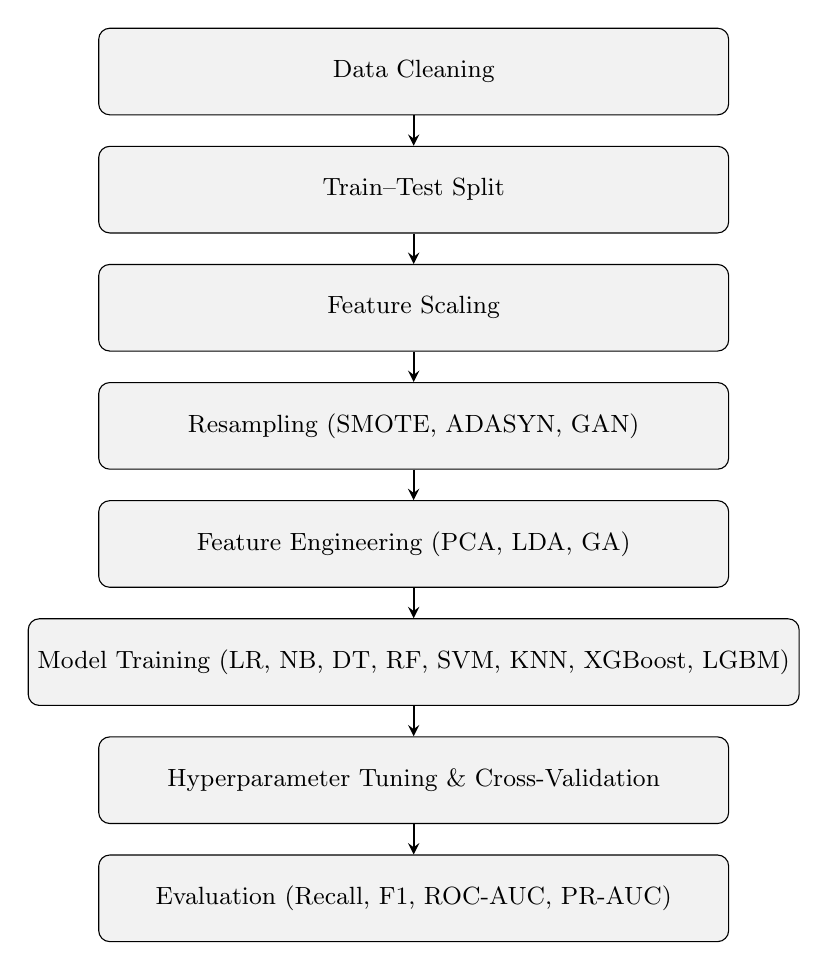
\begin{tikzpicture}[
        node distance=1.5cm,
        block/.style={
            rectangle,
            rounded corners,
            minimum width=8cm,
            minimum height=1.1cm,
            align=center,
            draw=black,
            fill=gray!10,
            font=\small
        },
        arrow/.style={thick,->,>=stealth}
    ]

    % Nodes
    \node (clean) [block] {Data Cleaning};

    \node (split) [block, below of=clean] {Train--Test Split};

    \node (scale) [block, below of=split] {Feature Scaling};

    \node (sample) [block, below of=scale] {Resampling (SMOTE, ADASYN, GAN)};

    \node (feat) [block, below of=sample] {Feature Engineering (PCA, LDA, GA)};

    \node (model) [block, below of=feat] {Model Training (LR, NB, DT, RF, SVM, KNN, XGBoost, LGBM)};

    \node (tuning) [block, below of=model] {Hyperparameter Tuning \& Cross-Validation};

    \node (eval) [block, below of=tuning] {Evaluation (Recall, F1, ROC-AUC, PR-AUC)};

    % Arrows
    \draw[arrow] (clean) -- (split);
    \draw[arrow] (split) -- (scale);
    \draw[arrow] (scale) -- (sample);
    \draw[arrow] (sample) -- (feat);
    \draw[arrow] (feat) -- (model);
    \draw[arrow] (model) -- (tuning);
    \draw[arrow] (tuning) -- (eval);

    \end{tikzpicture}

    \caption{Workflow of the Research Methodology}
    \label{fig:workflow}
\end{figure}